\section{Method and Data}\label{sec:data}

We describe the design of our randomized control experiment and the
dataset that we used for this experiment.

\subsection{Method}

In designing our controlled experiment, we follow the popular
statistical convention of experimental designers to refer to the service
upgrade as \factor{}, the group of users without the upgrade as
\control{} and the upgraded users as \treatment{}~\cite{stats-design}.

Controlled experiments are difficult to do on the Internet scale.  Our
work involves a randomized control experiment on the scale of a large
urban city. This enables us to study the effect of just one factor,
\emph{the service plan upgrade}, while other factors, such as price,
performance, or regional differences between users, are controlled. We
believe the affects observed on this dataset will also be observed in
others collected from urban cities and high tiers.

By examining a single ISP's high-capacity tier with an unannounced upgrade,
our dataset mitigates several biases that previous studies may have 
suffered. Studying the behavior of users who opt for buying a higher service plan
(unsatisfied subscribers) will naturally show an increase in demand on
upgrading service\cite{dasu-imc2014}.
Similarly users who have been offered an
upgrade in service may change their behavior to utilize the upgraded capacity
(cognitive bias)\cite{zheleva2013}. Studying datasets with these biases are prone 
to positive high correlation between demand and capacity. 

\begin{table}[t]
\small
\begin{tabular}{ l l }
\hline
\textbf{Field}         & \textbf{Description}				\\\hline
Device\_number         & Arbitrarily assigned household identifier	\\
end\_time              & 15 minute sample period end time		\\
cmts\_inet             & Anonymous IP identifier			\\
service\_direction     & \{downstream, upstream\}                 	\\
octets\_passed         & Byte count in 15 minutes sample period		\\\hline
\end{tabular}
\caption{Field descriptions for the \control{} and \treatment{} datasets.}
\label{tab:field-description}
\end{table}

\begin{figure*}[t]
\centering
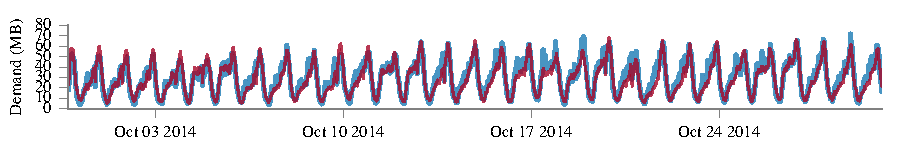
\includegraphics[width=\linewidth]{figures/traffic_demand_Oct.pdf}
  \caption{Traffic demand for an average subscriber in the \control{} and 
\treatment{} groups during October.\label{fig:traffic-load}}
\end{figure*}


\subsection{Data}

Our dataset consists of network usage byte counters reported every 15
minutes from October 1, 2014 to December 29, 2014 from about 22k
Comcast residential broadband gateways in Salt Lake City, Utah. Each
dataset contains the following fields: Device ID, the 15-minute time interval,
service class, service direction, anonymized IP address, and the bytes
transferred in each 15-minute interval, as described in
Table~\ref{tab:field-description}.

We divided the users into two groups: a \control{} set, consisting of
18,322 households with a 105 Mbps access link; and a \treatment{} set,
consisting of 2,219 households that were paying for a 105 Mbps access
link, yet were receiving 250 Mbps instead.  Subscribers in the
\treatment{} set were selected randomly and were not told that their
access bandwidth had been increased.  Our initial analysis of the data
from more than 22,000 households showed that not all gateways were
reporting their traffic counters every 15 minutes over the whole three-month
period: 32\% of the \treatment{} set, and 72\% of the \control{} set
gateway devices were responsive for less than 80\% of the time. For the
analysis in \autoref{sec:analysis}, we present our results based on the
accepted group of subscribers that contributed to the three-month dataset
more that 80\% during their lifetime. Our final sanitized dataset consisted of
4,845 subscribers in the \control{} group and 1,519 subscribers in the
\treatment{}.


\begin{table*}[t]
\begin{tabular}{| ccc|cccc|c |}
\hline
\multicolumn{3}{| c |}{} & \multicolumn{4}{c |}{Hourly traffic per 1000 subscribers} & \multicolumn{1}{c |}{per subscriber}\\ 
Dataset   & Direction & Subscribers & Total GBytes & 95\% Traffic & \textbf{PT 
Traffic} & \textbf{Non-PT Traffic} & Daily Demand \\ \hline
control   & downstream      & 4845         & \num{2.67e+5}               
   & 234.5  & \textbf{205.1}  & \textbf{108.5}       & 2.97   \\
treatment & downstream      & 1519         & \num{2.95e+5}  
& 244.42  & \textbf{209.5}  & \textbf{122.3}   & 3.30  \\\specialrule{0.005em}{0em}{0em} 
control   & upstream        & 4845        & \num{2.98e+4}  
& 21.39  & \textbf{18.942}  & \textbf{12.80}  & 0.33 \\
treatment & upstream        & 1519        & \num{4.27e+4} 
& 31.48   & \textbf{22.81}   & \textbf{19.02} & 0.48 \\\hline                                
\end{tabular}
\caption{Overview of the \control{} and \treatment{} datasets. The 95 
percentile traffic is the peak of total demand. PT traffic is the average 
traffic demand during prime-time hours. Non-PT traffic is calculated 
during non-prime-time. The daily demand is the average traffic demand per 
subscriber over a single day. All values are in Giga Bytes (GB).\label{tab:data-stats}}
\end{table*}



Figure \ref{fig:traffic-load} shows the downlink traffic demand per
subscriber (bytes per 15-minute sample period) for the month of October 
for both groups. The observed demand is diurnal, and reaches a peak daily
in the evening hours. Table \ref{tab:data-stats} compares the total demand
for subscribers in the \control{} and \treatment{} groups, scaled to a
thousand households. The downlink 95th percentile traffic demand 
over an hour is 234.5~GB for the lower tier \control{} group, and 244.42~GB
for the higher tier \treatment{} group.  Table \ref{tab:data-stats} also 
shows that an average subscriber
in the lower tier would download 2.97~GB in a day, and 3.30~GB if
they belonged to the higher tier. As for the uplink, an average
subscriber would transfer 0.33~GB in a day in the \control{} group, and
0.48~GB in a day in the \treatment{} group.

% The Service Level Agreement for subscribers with Comcast
% was 105 Mbps and the average subscribers does not fill the link
% consistently for 15 minutes to use the full capacity.